\documentclass[12pt]{article}

\usepackage{color}
\usepackage{graphicx}
\usepackage{amsmath}
\usepackage{float}
\usepackage{color}
\usepackage{indentfirst}
\usepackage{textcomp}
\usepackage{pifont}
\usepackage{multirow}
\usepackage{geometry}
\usepackage{algorithm}
\usepackage{algpseudocode}
\usepackage{amssymb}
\usepackage{algorithmicx}
\usepackage{amsmath} 
\usepackage{amsfonts}

\usepackage{listings}
\usepackage{xcolor}

\geometry{left = 2cm, right = 2cm, top = 3cm, bottom = 3cm}

\lstset{numbers=left,
        numberstyle=\tiny,
        keywordstyle=\color{blue}, 
        commentstyle=\color[cmyk]{1,0,1,0}, 
        frame=single, 
        escapeinside=``, 
        extendedchars=false, 
        xleftmargin=2em,xrightmargin=2em, aboveskip=1em, 
        tabsize=4, 
        showspaces=false 
       }

\floatname{algorithm}{Algorithm}
\renewcommand{\algorithmicrequire}{\textbf{Input:}}
\renewcommand{\algorithmicensure}{\textbf{Output:}}





\begin{document}

\vspace*{0.25cm}

\hrulefill

\thispagestyle{empty}

\begin{center}
\begin{large}
\sc{UM--SJTU Joint Institute \vspace{0.3em} \\ Bayesian Analysis \\ (VE414)}
\end{large}

\hrulefill

\vspace*{5cm}
\begin{Large}
\sc{{Assignment 1 \\ ~\\ }}
\end{Large}
\vspace{2em}

\end{center}


\vfill
\begin{large}

\begin{table}[h!]
\flushleft
\begin{tabular}{lll}
Name: Wu Guangzheng \hspace*{2em}\\
Student ID: 515370910014

\end{tabular}
\end{table}
\end{large}
\newpage
\begin{flushleft}


\section{Question 1} 

\subsection*{a)}

\qquad Let $A =  \text{The lower face of the coin is a head}$. 

\qquad Let $A_{11} =  \text{Picks a double-headed coin}$.

\qquad Let $A_{12} =  \text{A double-headed coin with a head at the bottom}$.

\qquad Let $A_{21} =  \text{Picks a double-tailed coin}$.

\qquad Let $A_{22} =  \text{A double-tailed coin with a head at the bottom}$.

\qquad Let $A_{31} =  \text{Picks a normal coin}$.

\qquad Let $A_{32} =  \text{A normal coin with a head at the bottom}$.

\vspace{-0.5cm}

\begin{align*}
P(A) &= P(A_{11}) \cdot P(A_{12}) + P(A_{21}) \cdot P(A_{22}) + P(A_{31}) \cdot P(A_{32})\\
&= 0.4 \cdot 1 + 0.2 \cdot 0 + 0.4 \cdot 0.5 = 0.6
\end{align*}


\subsection*{b)}

\qquad Let $B = \text{Opens his eye and finds a coin with a head on the top}$.

\vspace{-0.5cm}

\begin{align*}
P(A \mid B) = \frac{P(A, B)}{P(B)} = \frac{P(A_{11})}{P(B)} = \frac{0.4}{0.6}  = 0.667
\end{align*}

\subsection*{c)}


\qquad Let $B_{1} = \text{First throw with a head on the top.}$

\qquad Let $B_{2} = \text{Second throw with a head on the top.}$

\vspace{-0.5cm}

\begin{align*}
P(A\mid B_{1}, B_{2}) &= \frac{P(A, B_{1}, B_{2})}{P(B_{1}, B_{2})}\\
&= \frac{P(A_{11})}{P(A_{11}) \cdot P(A_{12})^2+ P(A_{21}) \cdot P(A_{22})^2 + P(A_{31}) \cdot P(A_{32})^2}\\
&= \frac{0.4}{0.5} = 0.8
\end{align*}

\newpage

\section{Question 2}

\qquad Let $X_i = j$ be the random variable that $j$ heads are shown in $i$ throws. \\

~\\

\qquad We define the likelihood of the coin throwing as

$$
L(p; x) = f_{X\mid P}(x\mid p) = \frac{k!}{x!(k-x)!}p^x(1-p)^{k-x}
$$

\qquad Thus we have

$$
L(p;x < 3) = f_{X\mid P}(x < 3\mid p) = \sum_{x=0}^2\frac{10!}{x!(10-x)!}p^x(1-p)^{10-x}
$$

\qquad And we know that 

\vspace{-0.5cm}

\begin{align*}
f_{P\mid X}(p\mid x)&\propto L(p; x<3) f_P(p)\\
&\propto (45\cdot p^2(1-p)^8 + 10\cdot p(1-p)^9 + (1-p)^{10}) \cdot (p^3(1-p)^3)\\
&\propto 45\cdot p^5(1-p)^{11} + 10\cdot p^4(1-p)^{12} + p^3(1-p)^{13}
\end{align*}

\qquad With calculation by mathematica, we get

$$
c = 7735 / 8
$$

\begin{figure*}[h]
\centering
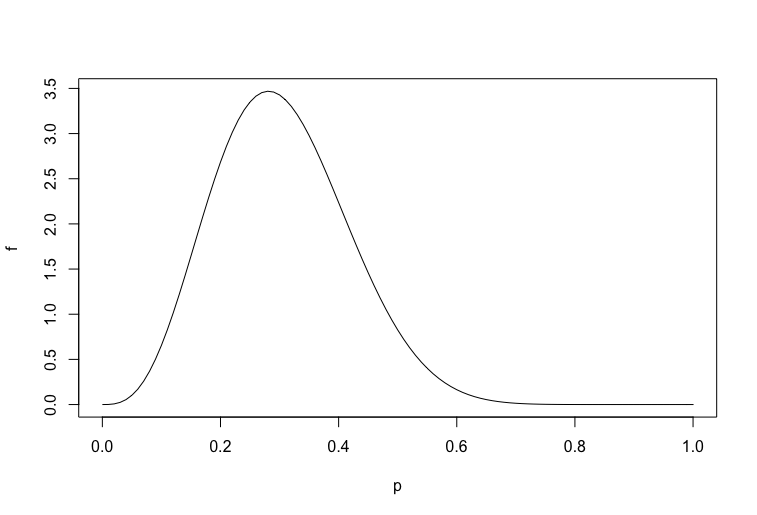
\includegraphics[width = 0.7\linewidth]{Ex2.png}
\end{figure*}

\newpage

\section{Question 3}

\subsection*{a)}

\qquad We use R to calculate the credible interval.

\begin{lstlisting}[language=R]
    a.prior = 1
    b.prior = 1

    a.posterior = a.prior + 40
    b.posterior = b.prior + 10
    l = qbeta(0.025, a.posterior, b.posterior) 
    u = qbeta(0.975, a.posterior, b.posterior)

    cat(paste("(",l, sep = ""), 
        paste(u,")", sep =""), 
        "\n", sep = ",")

\end{lstlisting} 

\qquad And we get the result that the credible interval for choosing F is $(0.669, 0.887)$. It shows that the choice of the people a biased towards F.

\subsection*{b)}


\qquad We use R to calculate the credible interval.

\begin{lstlisting}[language=R]
    a.prior = 1
    b.prior = 1

    a.posterior = a.prior + 15
    b.posterior = b.prior + 35
    l = qbeta(0.025, a.posterior, b.posterior) 
    u = qbeta(0.975, a.posterior, b.posterior)

    cat(paste("(",l, sep = ""), 
        paste(u,")", sep =""), 
        "\n", sep = ",")

\end{lstlisting} 

\qquad And we get the result that the credible interval for choosing F is $(0.191, 0.438)$. It shows that the choice of the people a biased towards J.


\section{Question 4}

\subsection*{a)}

\qquad We have 

$$
f_{X\mid P}(x\mid p) = p(1-p)^{x-1}
$$

\qquad So the likelihood should be 

$$
L(p; x) = \Pi_{i=1}^n f_{X_i \mid P}(x_i \mid p) = p^n(1-p)^{(\sum x_i) - n}
$$

\qquad Then we have the log likelihood

$$
l = \log L(p;x) = n\ln p + (-n +\sum x_i) \ln (1-p)
$$

\qquad To calculate the estimator, we should let the derivative to be 0

$$
\frac{\partial l(p;x)}{\partial p} = 0 \longrightarrow \frac{n}{p} - \frac{\sum x_i - n}{1-p} = 0
$$

\qquad So

$$
\hat{p} =\frac{n}{\sum x_i}
$$

\subsection*{b)}

\qquad Since

$$
q = p(1-p)
$$

\qquad So

$$
\hat{q} = \hat{p}(1-\hat{p}) = \frac{n}{\sum x_i}(1- \frac{n}{\sum x_i})
$$

\subsection*{c)}

\qquad Suppose a uniform prior, so the prior can also be the beta distribution

$$
p \sim \text{Beta}(1,1)
$$

\qquad Thus we have

\vspace{-0.5cm}

\begin{align*}
f_{P\mid X}(p\mid x) &\propto L(p;x) \cdot f_{P}(p) \propto p^{n}(1-p)^{- n + \sum x_i}
\end{align*}

\qquad So the posterior is still a Beta Distribution, with

$$
p \mid x \sim \text{Beta}(n+1 , -n + 1 + \sum x_i )
$$

\end{flushleft}
\end{document}